% =====================================================================
%  Comparative Risk Detection Across Banking Problems
%  Two-column, IEEE-style layout (article class, compiles with pdflatex)
% =====================================================================
\documentclass[10pt,twocolumn,a4paper]{article}

\usepackage[T1]{fontenc}
\usepackage[utf8]{inputenc}
\usepackage{mathptmx}
\usepackage[scaled=0.9]{helvet}
\usepackage[margin=0.75in,top=0.8in,bottom=0.85in,columnsep=0.25in]{geometry}
\usepackage{microtype}
\usepackage{amsmath,amssymb}
\usepackage{graphicx}
\usepackage{booktabs}
\usepackage{array}
\usepackage{multirow}
\usepackage{enumitem}
\usepackage{titlesec}
\usepackage{caption}
\usepackage{xcolor}
\usepackage{url}
\usepackage[colorlinks=true,linkcolor=black,citecolor=black,urlcolor=black]{hyperref}

\captionsetup{font=small,labelfont=bf,labelsep=period,justification=justified,singlelinecheck=false}
\captionsetup[table]{labelfont=bf,textfont=sc,labelsep=newline,justification=centering,singlelinecheck=true,skip=4pt}
\setlength{\parskip}{0pt}
\setlength{\parindent}{1.0em}
\setlist{nosep,leftmargin=1.4em,itemsep=1pt}
\setlength{\textfloatsep}{8pt plus 2pt minus 2pt}
\setlength{\floatsep}{8pt plus 2pt minus 2pt}
\setlength{\intextsep}{8pt plus 2pt minus 2pt}
\renewcommand{\arraystretch}{1.12}
\urlstyle{same}

%    IEEE-like headings                      -
\renewcommand{\thesection}{\Roman{section}}
\renewcommand{\thesubsection}{\Alph{subsection}}
\titleformat{\section}{\centering\normalfont\small\scshape}{\thesection.}{0.6em}{}
\titleformat{\subsection}{\normalfont\small\itshape}{\thesubsection.}{0.6em}{}
\titlespacing*{\section}{0pt}{10pt plus 2pt minus 2pt}{5pt}
\titlespacing*{\subsection}{0pt}{6pt plus 1pt minus 1pt}{3pt}
\renewcommand{\figurename}{Fig.}
\renewcommand{\tablename}{Table}
\renewcommand{\thetable}{\Roman{table}}

\newcommand{\pct}{\,\%}
\newcommand{\prauc}{PR-AUC}
\newcommand{\rocauc}{ROC-AUC}

\begin{document}

% =====================================================================
%  TITLE BLOCK
% =====================================================================
\twocolumn[{%
\begin{center}
{\fontsize{19}{22}\selectfont\bfseries Comparative Risk Detection Across Banking Problems:\\[2pt]
Fraud, Money Laundering and Customer Churn\par}
\vspace{10pt}
{\small
\begin{tabular}{@{}c@{\hspace{1.6em}}c@{\hspace{1.6em}}c@{\hspace{1.6em}}c@{}}
\textbf{Borshon Dopho} & \textbf{M. A. Al Nahian} & \textbf{Fahim Faysal} & \textbf{Jakia Tunnesa Rifa}\\
ID: 011221337 & ID: 011201416 & ID: 0112230224 & ID: 0112230469
\end{tabular}\\[4pt]
\itshape Department of Computer Science \& Engineering, United International University, Dhaka, Bangladesh}
\vspace{10pt}
\end{center}

\begin{center}
\begin{minipage}{0.92\textwidth}
\small\noindent\textbf{\textit{Abstract}}%
\newline
Banks are facing several distinct risks, including fraudulent transactions, money laundering and customer attrition, yet each is usually studied in isolation with its own model and evaluation protocol. This paper compares Decision Tree, Random Forest and XGBoost classifiers on three publicly available banking datasets: PaySim (fraud, 6.36M transactions), SAML-D (money laundering, 9.50M transactions) and a Botswana bank customer churn dataset (115,640 customers) using one shared experimental framework. The framework combines dataset-specific feature engineering, leakage control, a 70/30 train test split, SMOTE applied only inside the training folds of a stratified five-fold cross-validation, and model selection by \prauc{} followed by F1-score. The selected models are then evaluated once on an untouched test set. Random Forest was selected for PaySim (test F1 $=99.98\pct$, \prauc{} $=99.99\pct$), and XGBoost for SAML-D (F1 $=82.38\pct$, \prauc{} $=93.59\pct$) and churn (F1 $=97.71\pct$, \prauc{} $=99.86\pct$). The SAML-D result shows a clear precision recall trade-off (precision $74.13\pct$, recall $92.70\pct$) that overall accuracy ($99.96\pct$) completely hides. The results indicate that no single model is guaranteed to be best across banking risks: the most suitable choice depends on the dataset, the nature of the risk, and the balance between missed cases and false alarms.

\medskip
\noindent\textbf{\textit{Index Terms}}
fraud detection, anti-money laundering, customer churn, class imbalance, SMOTE, XGBoost, Random Forest, precision recall.
\end{minipage}
\end{center}
\vspace{6pt}
}]

% =====================================================================
\section{Introduction}
Banks operate under several kinds of risk at once. Fraudulent transactions cause direct financial loss, money laundering exposes institutions to regulatory and reputational damage, and customer churn erodes long-term revenue. Machine learning is widely used to flag all three, but the problems differ sharply in what a ``positive'' case looks like, how rare it is, and what a wrong prediction costs. A missed fraud or laundering case is expensive, while a false alarm consumes analyst time; in churn prediction, in contrast, a false alarm often only costs a retention offer.

A common difficulty is \emph{class imbalance}. In the two transaction datasets studied here, fewer than $0.13\pct$ of records are positive, so a classifier that labels everything as legitimate would be more than $99.8\pct$ accurate while detecting nothing. Accuracy is therefore a poor yardstick, and the precision recall trade-off is what matters in practice~\cite{davis2006,saito2015}.

Most published work treats fraud, anti-money-laundering (AML) and churn separately (see, e.g., \cite{mulyana2025,oztas2025,andespa2025}), which makes it hard to say whether conclusions about a model carry over from one risk to another. This study addresses that gap with a controlled comparison. The same three algorithms, the same imbalance-handling strategy, the same validation scheme and the same metrics are applied to three banking problems, so that differences in performance can be attributed mainly to the data and the risk rather than to the experimental setup.

Our research question is \emph{"How effectively can machine-learning models detect different types of banking risk, and how does their performance vary across fraud detection, money laundering detection and customer churn prediction?"}. In this paper, we test three models (Decision Tree, Random Forest and XGBoost) on three banking problems: fraud, money laundering and customer churn. We use the same steps for all three so the results are fair to compare. We choose the best model using PR-AUC and F1-score instead of accuracy, because the data is very imbalanced. We also look at how long training takes, what false alarms and missed cases mean in practice, and where our results should be treated with care.

% =====================================================================
\section{Background and Related Work}
\subsection{Risk Detection in Banking}
Fraud detection, AML monitoring and churn prediction are all supervised binary classification problems on tabular data, but they differ in structure. Fraud detection is a transaction-level problem in which signals such as inconsistent balance changes or unusual transaction types matter. AML monitoring is concerned with patterns of movement across accounts, and is typically evaluated at the transaction level when labels are available. Churn prediction operates at the customer level and relies on tenure, product holdings, balances and service history.

\subsection{Class Imbalance and Resampling}
Learning from imbalanced data is a well-studied problem~\cite{he2009}. The Synthetic Minority Over-sampling Technique (SMOTE) creates new minority examples by interpolating between a minority sample and its nearest minority neighbours~\cite{chawla2002}. Resampling must be applied only to training data; if it is applied before splitting or before cross-validation, synthetic points derived from validation records can leak into training and inflate scores. In this study SMOTE is therefore placed inside the cross-validation pipeline.

\subsection{Tree-Based Classifiers}
Decision trees~\cite{breiman1984} are interpretable but high-variance. Random Forests~\cite{breiman2001} average many decorrelated trees and are robust on tabular data. Gradient-boosted trees, of which XGBoost~\cite{chen2016} is a widely used implementation, build trees sequentially to correct earlier errors and often achieve the best accuracy on structured data. These three models span the range from an interpretable baseline to a strong ensemble.

\subsection{Evaluation Under Imbalance}
Because the precision recall curve focuses on the positive class, it is generally more informative than the ROC curve on heavily imbalanced data~\cite{saito2015,davis2006}. We therefore use the area under the precision recall curve (\prauc{}), computed as average precision, as the primary selection metric, with F1-score as the tie-breaker, and report \rocauc{}, precision, recall and accuracy for completeness.

\subsection{Datasets in the Literature}
PaySim is a simulator of mobile-money transactions built from aggregated real logs~\cite{lopez2016}. SAML-D is a synthetic transaction-monitoring dataset created to support AML research, with labelled laundering typologies~\cite{oztas2023}. The Botswana bank customer churn dataset is publicly distributed through Kaggle~\cite{mfazi}. Using these three together allows a like-for-like comparison across risk types.

\subsection{Related Work}
One study compared Decision Tree, Random Forest and XGBoost on PaySim using random undersampling. Random Forest was the most accurate (about $99\%$), followed by XGBoost ($98.9\%$) and Decision Tree ($97\%$)~\cite{mulyana2025}. Another study oversampled PaySim and compared Logistic Regression, Gradient Boosting and XGBoost, where XGBoost performed best (accuracy $99.88\%$) and threshold moving was used to tune detection~\cite{doddamani2024}. A third study combined a Local Outlier Factor stage with LightGBM and SMOTE on PaySim~\cite{tetik2025}. On a credit-card fraud dataset, Random Forest and XGBoost with SMOTE outperformed the other classifiers, and the authors noted that the age of the data limits generalization~\cite{andrade2025}.

For money laundering, a transformer-based model tested on SAML-D reached an ROC-AUC of $93.01$ with a $98\%$ true-positive rate and a $51\%$ false-positive rate, and it outperformed TabTransformer and XGBoost~\cite{oztas2025}. An interview study with eight AML specialists found that rule-based transaction monitoring produces many false positives, and it suggested graph analysis and anomaly detection as improvements~\cite{oztas2024}.

For churn, a comparison of Random Forest and XGBoost on a bank dataset with SMOTE and SMOTE-ENN found that XGBoost with SMOTE was best (F1 $=0.873$, AUC $=0.983$)~\cite{andespa2025}. Another study varied the churn rate from $15\%$ to $1\%$ in a telecom setting. XGBoost with SMOTE gave the highest F1-score at every imbalance level, while Random Forest performed poorly under severe imbalance~\cite{imani2025}.

Each of these studies covers a single risk domain, and some rely on random splits~\cite{mulyana2025,andrade2025}. Our work applies one leakage-aware protocol to all three domains, with time-ordered splits for the transaction data, so the domains can be compared directly.

% =====================================================================
\section{Datasets}
Table~\ref{tab:datasets} summarizes the three datasets, and Fig.~\ref{fig:imbalance} compares their positive-class rates. PaySim and SAML-D are extremely imbalanced ($0.129\pct$ and $0.104\pct$ positive), whereas churn is moderately imbalanced ($12.19\pct$).

\begin{table}[t]
\centering
\caption{Dataset Overview}
\label{tab:datasets}
\footnotesize
\setlength{\tabcolsep}{3.2pt}
\begin{tabular}{@{}lccc@{}}
\toprule
 & \textbf{PaySim} & \textbf{SAML-D} & \textbf{Churn}\\
\midrule
Risk problem & Fraud & Laundering & Churn\\
Records & 6,362,620 & 9,504,852 & 115,640\\
Positive cases & 8,213 & 9,873 & 14,094\\
Positive rate & 0.129\% & 0.104\% & 12.19\%\\
Train records & 4,453,834 & 6,653,396 & 80,948\\
Test records & 1,908,786 & 2,851,456 & 34,692\\
Train positives & 3,643 & 6,764 & 9,866\\
Test positives & 4,570 & 3,109 & 4,228\\
Train / test rate & 0.082 / 0.239\% & 0.102 / 0.109\% & 12.19 / 12.19\%\\
Split type & Chronological & Chronological & Stratified\\
\bottomrule
\end{tabular}

\end{table}

\begin{figure}[t]
\centering
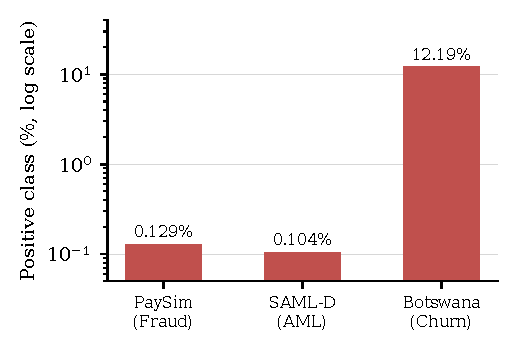
\includegraphics[width=0.88\columnwidth]{figures/fig_imbalance.pdf}
\caption{Positive-class rate in each dataset (log scale). Fraud and laundering cases are roughly two orders of magnitude rarer than churn cases.}
\label{fig:imbalance}
\end{figure}

Each record is a mobile-money transaction with a time step (hour), transaction type, amount, origin and destination balances before and after the transaction, and a fraud label. The original \texttt{isFlaggedFraud} field was removed, as it is a rule-based flag generated by the simulator rather than an input feature. No missing values or duplicates were found.

Each record is a transaction with date, time, sender and receiver accounts, amount, payment and received currency, sender and receiver bank locations, payment type, a laundering label, and a laundering-typology label. The typology label was excluded, since it only exists for laundering cases and would leak the target.

Each record is a customer with demographic attributes, income, tenure, credit information, outstanding loans, balance, number of products and complaints, and a churn flag. \texttt{Churn Reason} and \texttt{Churn Date} are populated only for churned customers (101,546 missing values, equal to the number of retained customers) and were removed to prevent target leakage.

% =====================================================================
\section{Methodology}
Fig.~\ref{fig:pipeline} shows the pipeline applied to every dataset. The same sequence of steps is used throughout; only the feature engineering and a small number of model settings are dataset-specific.

\begin{figure*}[t]
\centering
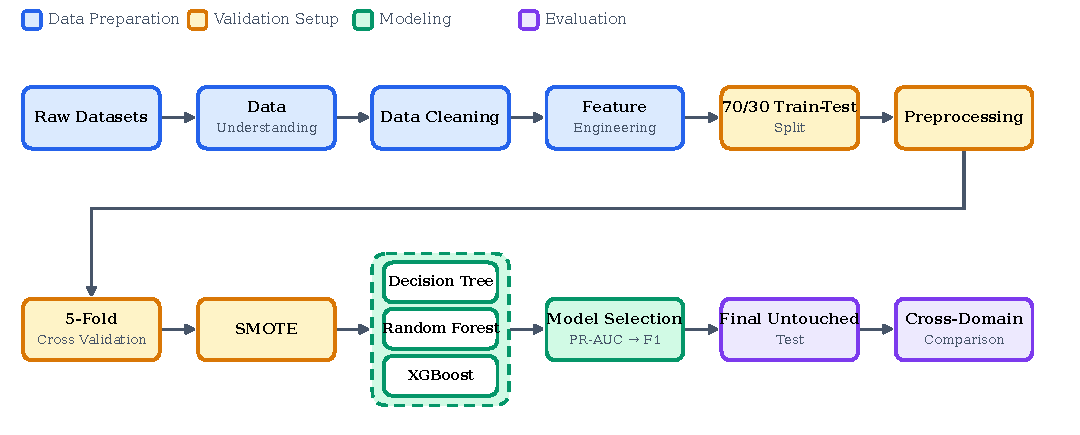
\includegraphics[width=0.92\textwidth]{figures/fig_pipeline.pdf}
\caption{Overview of the methodology pipeline shared by all three banking problems, from raw data through preprocessing, SMOTE-based cross-validation, model selection and the final untouched test.}
\label{fig:pipeline}
\end{figure*}

\subsection{Feature Engineering}
Features were designed per dataset to capture the signals most relevant to each risk (Table~\ref{tab:features}). Identifiers (account names, customer IDs, names, addresses and contact details) were removed.

\begin{table*}[t]
\centering
\caption{Engineered Features and Leakage Controls per Dataset}
\label{tab:features}
\footnotesize
\setlength{\tabcolsep}{4pt}
\begin{tabular}{@{}>{\raggedright\arraybackslash}p{0.095\textwidth}>{\raggedright\arraybackslash}p{0.54\textwidth}>{\raggedright\arraybackslash}p{0.30\textwidth}@{}}
\toprule
\textbf{Dataset} & \textbf{Engineered features} & \textbf{Removed (leakage / identifiers)}\\
\midrule
PaySim &
Origin and destination balance errors ($\text{old}-\text{amount}-\text{new}$ and $\text{old}+\text{amount}-\text{new}$); zero-balance flags; log transforms of amount and balances; amount-to-balance ratios; running transaction counts for sender and receiver; same-account flag; transfer/cash-out flag. (1 categorical + 21 numerical features.) &
Sender and receiver names, \texttt{isFlaggedFraud}.\\
\addlinespace
SAML-D &
Currency mismatch; bank-location mismatch and same-location flag; log amount and zero-amount flag; hour, day of week and weekend flag; running counts for sender, receiver and sender receiver pair. (5 categorical + 12 numerical features.) &
\texttt{Laundering\_type}, sender and receiver accounts, raw date and time.\\
\addlinespace
Churn &
Age (from date of birth); balance-to-income and loan-to-income ratios; log of balance, income and loans; products per tenure; balance per product; complaints per tenure. (6 categorical + 18 numerical features.) &
\texttt{Churn Reason}, \texttt{Churn Date}, IDs, names, address, contact information, date of birth.\\
\bottomrule
\end{tabular}
\end{table*}

In PaySim and SAML-D the running counts are computed with a cumulative count over the chronologically sorted data, so each record only sees earlier activity of the same account and no information flows backwards from the future.

\subsection{Train Test Split}
The two transaction datasets are sorted by time and split chronologically, with the first 70\% used for training and the last 30\% for testing. This mimics deployment, where a model trained on the past scores future transactions. The churn dataset has no temporal ordering, so a stratified random 70/30 split (seed 42) was used, which preserves the 12.19\% churn rate in both partitions.

\subsection{Preprocessing and Imbalance Handling}
Categorical variables are one-hot encoded (unseen categories ignored). For PaySim and churn, numerical variables are standardized; for SAML-D they are passed through unchanged. SMOTE is then applied to the \emph{training portion of each fold only}, using an \texttt{imblearn} pipeline in which preprocessing, SMOTE and the classifier are fitted together, so validation folds are never resampled. The sampling ratio (minority-to-majority after resampling) was $0.1$ for PaySim and SAML-D, which are extremely imbalanced, and $0.5$ for churn. For PaySim, SMOTE used $k=5$ neighbours.

\subsection{Models}
Three classifiers are compared in every domain: a Decision Tree (interpretable baseline), a Random Forest (bagged ensemble) and XGBoost (gradient boosting). Their hyperparameters (Table~\ref{tab:hparams}) were fixed in advance and not tuned per dataset beyond adjusting tree depth and number of trees to dataset size. All use random seed 42.

\begin{table}[t]
\centering
\caption{Model Hyperparameters}
\label{tab:hparams}
\footnotesize
\setlength{\tabcolsep}{2.6pt}
\begin{tabular}{@{}llccc@{}}
\toprule
\textbf{Model} & \textbf{Setting} & \textbf{PaySim} & \textbf{SAML-D} & \textbf{Churn}\\
\midrule
\multirow{2}{*}{Decision Tree} & max depth & 12 & none & 10\\
 & min leaf samples & 10 & 2 & 10\\
\addlinespace
\multirow{3}{*}{Random Forest} & trees & 100 & 200 & 200\\
 & max depth & 20 & none & 20\\
 & min leaf samples & 5 & 2 & 5\\
\addlinespace
\multirow{4}{*}{XGBoost} & trees & 200 & 300 & 300\\
 & max depth & 6 & 6 & 6\\
 & learning rate & 0.10 & 0.10 & 0.05\\
 & subsample / colsample & 0.8 / 0.8 & 0.8 / 0.8 & 0.8 / 0.8\\
\midrule
SMOTE & sampling ratio & 0.1 & 0.1 & 0.5\\
\bottomrule
\end{tabular}
\end{table}

\subsection{Validation and Model Selection}
On each training set, stratified five-fold cross-validation (shuffled, seed 42) was run for all three models with SMOTE inside each fold. The model with the highest mean \prauc{} was selected, with F1-score used as the secondary criterion. The selected model was then retrained on the entire training set (with SMOTE) and evaluated exactly once on the held-out test set.

\subsection{Evaluation Metrics}
With true positives $TP$, false positives $FP$, false negatives $FN$ and true negatives $TN$:
\begin{equation}
\text{Precision}=\frac{TP}{TP+FP},\quad
\text{Recall}=\frac{TP}{TP+FN},
\end{equation}
\begin{equation}
F_1=\frac{2\cdot\text{Precision}\cdot\text{Recall}}{\text{Precision}+\text{Recall}}.
\end{equation}
Precision measures how many raised alerts are correct, and recall measures how many true cases are found. \prauc{} summarizes the precision recall trade-off across all thresholds, and \rocauc{} summarizes the true-positive versus false-positive trade-off. All thresholds for hard predictions are the default $0.5$ on predicted probability; no threshold tuning was performed.

% =====================================================================
\section{Results}
\subsection{Cross-Validation Comparison}
Table~\ref{tab:cv} reports the five-fold cross-validation results for all three models, and Fig.~\ref{fig:cvmodels} shows \prauc{} by model. The selected model in each domain is marked in bold.

\begin{table*}[t]
\centering
\caption{Five-Fold Cross-Validation Results (SMOTE inside folds). Mean over folds; selected model in bold.}
\label{tab:cv}
\footnotesize
\setlength{\tabcolsep}{5pt}
\begin{tabular}{@{}llccccccr@{}}
\toprule
\textbf{Dataset} & \textbf{Model} & \textbf{Acc.} & \textbf{Prec.} & \textbf{Rec.} & \textbf{F1} & \textbf{ROC-AUC} & \textbf{PR-AUC} & \textbf{CV time (s)}\\
\midrule
\multirow{3}{*}{PaySim}
 & Decision Tree & 0.99990 & 0.8952 & 0.9920 & 0.9407 & 0.9980 & 0.9897 & 571\\
 & \textbf{Random Forest} & \textbf{0.99998} & \textbf{0.9810} & \textbf{0.9915} & \textbf{0.9862} & \textbf{0.9991} & \textbf{0.9948} & \textbf{6,929}\\
 & XGBoost & 0.99999 & 0.9950 & 0.9909 & 0.9930 & 0.9992 & 0.9943 & 736\\
\midrule
\multirow{3}{*}{SAML-D}
 & Decision Tree & 0.99968 & 0.8965 & 0.7725 & 0.8298 & 0.8925 & 0.7205 & 448\\
 & Random Forest & 0.99965 & 0.9885 & 0.6634 & 0.7938 & 0.9939 & 0.8212 & 5,840\\
 & \textbf{XGBoost} & \textbf{0.99972} & \textbf{0.9824} & \textbf{0.7343} & \textbf{0.8404} & \textbf{0.9955} & \textbf{0.8267} & \textbf{2,464}\\
\midrule
\multirow{3}{*}{Churn}
 & Decision Tree & 0.9804 & 0.9033 & 0.9400 & 0.9212 & 0.9841 & 0.9428 & 39\\
 & Random Forest & 0.9545 & 0.7708 & 0.8923 & 0.8270 & 0.9863 & 0.9283 & 117\\
 & \textbf{XGBoost} & \textbf{0.9939} & \textbf{0.9682} & \textbf{0.9822} & \textbf{0.9751} & \textbf{0.9997} & \textbf{0.9982} & \textbf{155}\\
\bottomrule
\end{tabular}
\end{table*}

\begin{figure}[t]
\centering
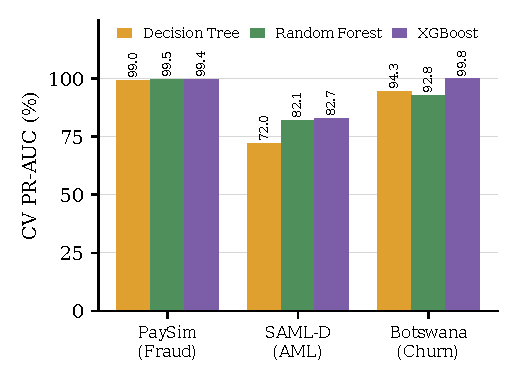
\includegraphics[width=\columnwidth]{figures/fig_cv_models.pdf}
\caption{Cross-validated \prauc{} of the three classifiers in each domain. XGBoost leads on SAML-D and churn; on PaySim, Random Forest and XGBoost are almost tied.}
\label{fig:cvmodels}
\end{figure}

On PaySim the top two models are very close: Random Forest has a mean \prauc{} of $0.9948$ versus $0.9943$ for XGBoost, a gap of $0.0005$. Random Forest was selected because the protocol ranks on \prauc{} first, even though XGBoost had a higher CV F1-score ($0.9930$ vs.\ $0.9862$) and higher precision, and ran about nine times faster ($736$ s vs.\ $6{,}929$ s). On SAML-D XGBoost had the best \prauc{}, \rocauc{} and F1, while Random Forest had the highest precision and the Decision Tree the highest recall. On churn XGBoost led on every metric, while Random Forest was clearly the weakest ($F_1=0.827$).

\subsection{Final Test Performance}
Table~\ref{tab:test} gives the held-out test results for the selected models, and Fig.~\ref{fig:prf} compares precision, recall and F1.

\begin{table*}[t]
\centering
\caption{Final Held-Out Test Performance of the Selected Model in Each Domain (\%)}
\label{tab:test}
\footnotesize
\setlength{\tabcolsep}{5pt}
\begin{tabular}{@{}llcccccccc@{}}
\toprule
\textbf{Dataset} & \textbf{Model} & \textbf{Acc.} & \textbf{Prec.} & \textbf{Rec.} & \textbf{F1} & \textbf{ROC-AUC} & \textbf{PR-AUC} & \textbf{Train (s)} & \textbf{Test (s)}\\
\midrule
PaySim (Fraud) & Random Forest & 99.9999 & 99.9781 & 99.9781 & 99.9781 & 100.0000 & 99.9999 & 1,812.9 & 19.6\\
SAML-D (AML) & XGBoost & 99.9568 & 74.1255 & 92.6986 & 82.3782 & 99.9475 & 93.5894 & 592.6 & 43.1\\
Churn & XGBoost & 99.4379 & 96.9718 & 98.4626 & 97.7115 & 99.9803 & 99.8634 & 43.0 & 0.6\\
\bottomrule
\end{tabular}
\end{table*}

\begin{figure}[t]
\centering
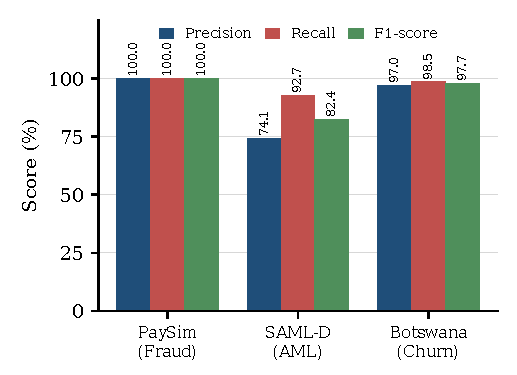
\includegraphics[width=\columnwidth]{figures/fig_test_prf.pdf}
\caption{Test precision, recall and F1-score of the selected model in each domain. Precision is the weak point on SAML-D.}
\label{fig:prf}
\end{figure}

PaySim and churn are detected almost perfectly. SAML-D is clearly harder: recall is high ($92.70\pct$), but precision is only $74.13\pct$, so about one in four alerts is a false alarm. Note that SAML-D accuracy is $99.96\pct$, higher than churn accuracy ($99.44\pct$), even though SAML-D is by far the weaker detector. This is a direct illustration of why accuracy is misleading under severe imbalance.

\subsection{Error Analysis}
Fig.~\ref{fig:cm} shows the confusion matrices. On PaySim only one legitimate transaction was flagged and one fraud missed among $1{,}908{,}786$ test records. On SAML-D, $2{,}882$ of $3{,}109$ laundering transactions were detected, $227$ were missed and $1{,}006$ legitimate transactions were flagged. On churn, $4{,}163$ of $4{,}228$ churners were identified, with $65$ missed and $130$ false alarms.

\begin{figure*}[t]
\centering
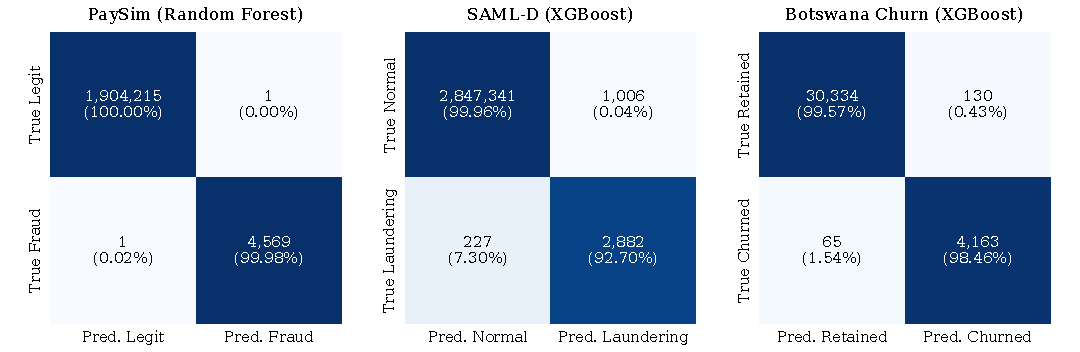
\includegraphics[width=0.95\textwidth]{figures/fig_confusion.pdf}
\caption{Confusion matrices on the held-out test sets (counts and row-normalized percentages).}
\label{fig:cm}
\end{figure*}

\subsection{Cross Validation Versus Test}
Fig.~\ref{fig:cvtest} compares cross-validated and test scores. Churn is stable (\prauc{} $0.9982\rightarrow0.9986$; F1 $0.9751\rightarrow0.9771$). PaySim improves on the test set (\prauc{} $0.9948\rightarrow0.9999$). SAML-D shows the largest shift: \prauc{} rises from $0.827$ to $0.936$, while F1 slightly falls ($0.840\rightarrow0.824$) and the balance of precision and recall changes completely (CV precision $0.982$ and recall $0.734$; test precision $0.741$ and recall $0.927$). This pattern is discussed in Section~\ref{sec:discussion}.

\begin{figure*}[t]
\centering
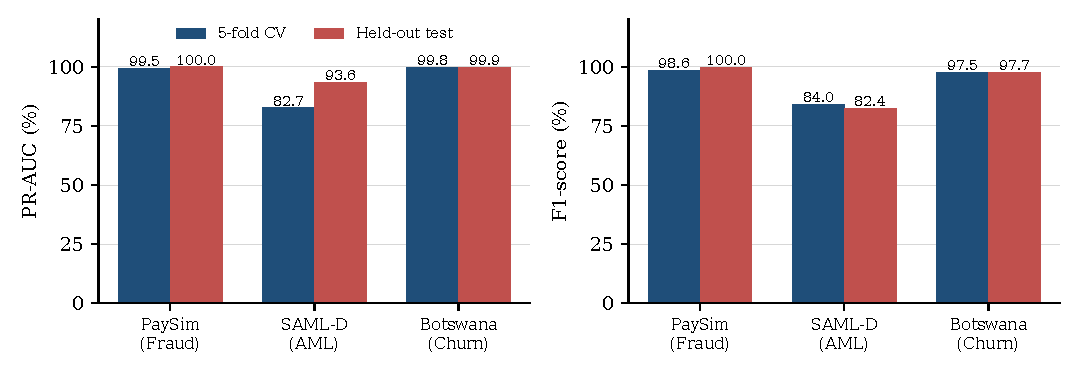
\includegraphics[width=0.95\textwidth]{figures/fig_cv_vs_test.pdf}
\caption{Cross-validation versus held-out test \prauc{} (left) and F1-score (right).}
\label{fig:cvtest}
\end{figure*}

% =====================================================================
\section{Discussion}
\label{sec:discussion}
Random Forest was selected for fraud, and XGBoost for money laundering and churn. The PaySim margin was very small, so the stronger claim is not that Random Forest is better for fraud but that the ranking of models was not the same in all three domains and that the size of the gap between them varies widely (large on churn, small on PaySim). This supports the central message that model choice should be made per problem.

Our churn results agree with recent work in which XGBoost with SMOTE was the strongest model and Random Forest degraded under imbalance~\cite{andespa2025,imani2025}: in our CV, XGBoost led on churn while Random Forest was weakest. The PaySim ordering (Random Forest $\geq$ XGBoost $>$ Decision Tree on \prauc{}) matches the ordering reported in~\cite{mulyana2025}, although their protocol (undersampling, random split) differs from ours. The Tab-AML result on SAML-D~\cite{oztas2025} is not directly comparable to ours, because the split, features and operating point differ; it does, however, point to the same difficulty we observe, namely a trade-off between detecting laundering and generating false alerts.

PaySim's engineered balance-error features expose a strong, almost deterministic signature of fraud in the simulated data, which likely explains the near-perfect test scores; whether real-world fraud is as separable is not something this experiment can show. Churn benefits from informative customer-behaviour features and a moderate $12.19\pct$ positive rate. SAML-D is the hardest: laundering is defined by patterns across accounts and time, while the features used here are mostly transaction-level, so many laundering transactions look ordinary in isolation. Richer network or time-window features are a natural next step.

On SAML-D, 1,006 false alerts accompany 2,882 true detections. For an AML team this is roughly $0.35$ false alert per correct one, which may be acceptable if missing laundering is much costlier than reviewing an alert, but it must be a deliberate choice. A decision threshold other than $0.5$ could trade recall for precision; this was not explored. On churn, the cost of a false positive (an unnecessary retention offer) is low, so the high recall is appropriate.

In cross-validation SAML-D had high precision ($0.98$) and modest recall ($0.73$); on the test set the pattern reversed. We have not isolated the cause. Two plausible contributors are that cross-validation shuffles chronologically ordered training data while the test set is a later time period, and that the laundering mix may differ between periods. This is a reason to treat the SAML-D CV numbers as a guide to model ranking rather than as an estimate of test performance.

Accuracy exceeded $99.4\pct$ in all three domains, but F1 ranged from $82.4\pct$ to $99.98\pct$. \prauc{}, precision and recall expose differences that accuracy hides, supporting the use of \prauc{} for selection.
\newline
\newline
\newline
\newline
\newline
\newline
\newline
\newline
\newline
\newline
\newline
\newline
\newline
\newline
\newline
\newline
\newline
\newline
\newline
\newline
\newline
\newline
\newline
\newline
\newline
\newline
\newline
\newline
\newline
\newline
\newline
\newline
\newline
\newline
\newline
\newline
\newline
% =====================================================================
\section{Limitations}
\begin{enumerate}
\item \textbf{Synthetic or simulated data:} PaySim and SAML-D are simulation-based, so performance may not transfer to production systems.
\item \textbf{Fixed Hyperparameters:} Hyperparameters were set once per dataset rather than tuned with a search, so the ranking of models could change under tuning.
\item \textbf{Single split and seed:} Results come from one train test split and one random seed, and no confidence intervals or significance tests are reported.
\item \textbf{Default decision threshold:} No threshold tuning or cost-sensitive analysis was done, although costs of false positives and negatives differ by domain.
\item \textbf{Shuffled CV on chronological data:} For PaySim and SAML-D, cross-validation inside the training period was shuffled rather than time-ordered, which may explain part of the CV-to-test differences.
\item \textbf{Transaction-level features for AML:} SAML-D features do not include graph or network features, which are central to laundering detection.
\item \textbf{No interpretability analysis:} Feature importance and explanations were not examined.
\end{enumerate}
% =====================================================================
\section{Future Work}
Future work should (i) tune hyperparameters with a proper search and report variance across seeds; (ii) use time-aware cross-validation for the transaction datasets; (iii) add graph-based and time-window features for AML; (iv) tune decision thresholds against explicit cost assumptions; (v) add interpretability analysis such as feature importance; (vi) compare SMOTE with class weighting and other resampling strategies; and (vii) validate on real or additional datasets.

% =====================================================================
\section{Conclusion}
This paper compared Decision Tree, Random Forest and XGBoost for fraud, money laundering and churn detection under one leakage-aware framework with SMOTE inside cross-validation and PR-AUC-based model selection. Random Forest was selected for PaySim and XGBoost for SAML-D and churn. Fraud and churn were detected with F1-scores of $99.98\pct$ and $97.71\pct$, while money laundering remained harder (F1 $82.38\pct$, precision $74.13\pct$, recall $92.70\pct$). Accuracy was above $99.4\pct$ in all cases and so could not distinguish the problems. The main conclusion is that performance and the best model are problem-specific: no model was universally best, and the right choice depends on the data, the risk, and the balance between missed cases and false alarms. The results should be interpreted within the stated limitations, in particular the simulated nature of two datasets and the near-perfect PaySim score.
\clearpage
% =====================================================================
\begingroup
\small
\renewcommand{\refname}{\centering\normalfont\small\scshape References}
\begin{thebibliography}{99}
\setlength{\itemsep}{1pt}

\bibitem{davis2006} J. Davis and M. Goadrich, ``The relationship between precision-recall and ROC curves,'' in \emph{Proc. 23rd Int. Conf. Machine Learning (ICML)}, 2006, pp. 233 240.

\bibitem{saito2015} T. Saito and M. Rehmsmeier, ``The precision-recall plot is more informative than the ROC plot when evaluating binary classifiers on imbalanced datasets,'' \emph{PLoS ONE}, vol. 10, no. 3, e0118432, 2015.

\bibitem{mulyana2025} I. Mulyana and M. B. Ulum, ``Application of machine learning models for fraud detection in synthetic mobile financial transactions,'' \emph{J. Ilmu Pengetahuan dan Teknol. Komput. (JITK)}, vol. 10, no. 4, pp. 759 768, May 2025.

\bibitem{oztas2025} B. Oztas, D. Cetinkaya, F. Adedoyin, M. Budka, H. Dogan, and G. Aksu, ``Tab-AML: A transformer based transaction monitoring model for anti-money laundering,'' in \emph{Proc. IEEE Conf. Artificial Intelligence (CAI)}, Santa Clara, CA, USA, 2025, pp. 161 167.

\bibitem{andespa2025} R. Andespa, K. Sadik, C. Suhaeni, and A. M. Soleh, ``Evaluating random forest and XGBoost for bank customer churn prediction on imbalanced data using SMOTE and SMOTE-ENN,'' \emph{Media Statistika}, vol. 18, no. 1, pp. 25 36, Oct. 2025.

\bibitem{he2009} H. He and E. A. Garcia, ``Learning from imbalanced data,'' \emph{IEEE Trans. Knowl. Data Eng.}, vol. 21, no. 9, pp. 1263 1284, 2009.

\bibitem{chawla2002} N. V. Chawla, K. W. Bowyer, L. O. Hall, and W. P. Kegelmeyer, ``SMOTE: Synthetic minority over-sampling technique,'' \emph{J. Artif. Intell. Res.}, vol. 16, pp. 321 357, 2002.

\bibitem{breiman1984} L. Breiman, J. H. Friedman, R. A. Olshen, and C. J. Stone, \emph{Classification and Regression Trees}. Belmont, CA, USA: Wadsworth, 1984.

\bibitem{breiman2001} L. Breiman, ``Random forests,'' \emph{Mach. Learn.}, vol. 45, no. 1, pp. 5 32, 2001.

\bibitem{chen2016} T. Chen and C. Guestrin, ``XGBoost: A scalable tree boosting system,'' in \emph{Proc. 22nd ACM SIGKDD Int. Conf. Knowledge Discovery and Data Mining}, 2016, pp. 785 794.

\bibitem{lopez2016} E. A. Lopez-Rojas, A. Elmir, and S. Axelsson, ``PaySim: A financial mobile money simulator for fraud detection,'' in \emph{Proc. 28th European Modeling and Simulation Symp. (EMSS)}, Larnaca, Cyprus, 2016.

\bibitem{oztas2023} B. Oztas, D. Cetinkaya, F. Adedoyin, M. Budka, H. Dogan, and G. Aksu, ``Enhancing anti-money laundering: Development of a synthetic transaction monitoring dataset,'' in \emph{Proc. IEEE Int. Conf. e-Business Engineering (ICEBE)}, 2023, pp. 47 54.

\bibitem{mfazi} S. D. Mfazi, ``Bank customer churn,'' Kaggle dataset.

\bibitem{doddamani2024} S. S. Doddamani, K. K. Girish, and B. Bhowmik, ``Money laundering detection in imbalanced e-wallet transactions with threshold optimization,'' in \emph{Proc. 9th IEEE Int. Conf. Convergence in Technology (I2CT)}, 2024.

\bibitem{tetik2025} A. Tetik and E. G\"{u}l, ``Fraud detection using machine learning in banking operations,'' in \emph{Proc. Innovations in Intelligent Systems and Applications Conf. (ASYU)}, Bursa, T\"{u}rkiye, 2025.

\bibitem{andrade2025} L. Andrade-Arenas and C. Yactayo-Arias, ``Comparative analysis of machine learning models for credit card fraud detection using SMOTE for class imbalance,'' \emph{Int. J. Saf. Secur. Eng.}, vol. 15, no. 5, pp. 893 901, May 2025.

\bibitem{oztas2024} B. Oztas, D. Cetinkaya, F. Adedoyin, M. Budka, G. Aksu, and H. Dogan, ``Transaction monitoring in anti-money laundering: A qualitative analysis and points of view from industry,'' \emph{Future Gener. Comput. Syst.}, vol. 159, pp. 161 171, 2024.

\bibitem{imani2025} M. Imani, A. Beikmohammadi, and H. R. Arabnia, ``Comprehensive analysis of random forest and XGBoost performance with SMOTE, ADASYN, and GNUS under varying imbalance levels,'' \emph{Technologies}, vol. 13, no. 3, art. 88, Feb. 2025.

\end{thebibliography}
\endgroup

\end{document}
